\chapter{Parameter Estimation}
\label{sec:Parameter estimation}

Identification of a model's parameters is an inverse problem. As such, identification consists in the characterization of the inputs and parameters of a system given the outputs and rest of the inputs of such system. Frequently, \textit{a priori} information on the system can be used to narrow the search path of the problem, but this type of information is not enough to allow for a complete derivation of the models. In the glucose-insulin model identification paradigm, the inverse problem is usually reduced to finding the parameters of a model which characterize an individual given the glucose profile of that patient, and the patients information such as meal characteristics and insulin treatments.

\section{Optimization and Intervals}
\label{sec:OptimizationAndIntervals}

Parameter estimation is usually posed as an optimization problem. Its solution relies on optimization algorithms attempting to optimize an index of the fit of the model's output to the available data. Usually scalar indexes are considered for characterizing the deviation of the model from the data. Such indexes can be formulated, for example, as a quadratic error depending on a set of parameters $p$ that has to be minimized:

\begin{equation}
	J(p)=\sum_{i=1}^{N}(y_{i}(p)-\tilde{y}_{i})^{T}Q_{i}(y_{i}(p)-\tilde{y}_{i})
\label{eq:quadraticindex}
\end{equation}

where $y_{i}(p)$ are the model predictions for time $i$ and $\tilde{y}_{i}$ are the experimental measurements, therefore, the data to be fitted. $Q_{i}$ is the data weighting matrix, which permits to fit more accurately some data in detriment to other data samples.  $Q_{i}$ is usually chosen as a diagonal matrix, due to the assumption that data samples are independently correlated to each other. The choice of the diagonal values in the matrix are usually referred to as ``weights'' of the data samples. This quadratic error index reflects the most classical approach to parameter estimation.

A usual compromise choice for the weighting matrix is to make the relative errors of each data sample weight the same in the cost index in order to fit all data points equally in the time axis. This is achieved by forcing the diagonal of $Q_{i}$ to be equal to $1/\tilde{y}_{i}^{2}$. This type of ponderation matrix has the disadvantage of underestimating large errors in high glucose values (hyperglycemic region) of the output of the model than in low values (hypoglycemic case). Usually it is preferred that all errors are normalized in the optimization index, and this is achieved with a different weighting matrix, like for example the case where all the elements of the diagonal are equal to $1/max(\tilde{y}_{i})^{2}$. This way the contribution of every data sample is standardized in the glucose concentration axis.

The most common choice of optimization methods for parameter estimation are simple local optimization algorithms, with iterative executions for easier convergence. There are many drawbacks to the use of local optimization:

\begin{enumerate}
	\item The initial value of the parameters to be chosen for the identification heavily influences the final outcome of the optimization. The choice of these values relies strongly in guesswork.
	\item Convergence to the global optimum of the problem is achievable, but not guaranteed.
	\item There may be several sets of parameters that yield similar optimization index values. This problem may happen with a very flat solution region but it can also happen for different local ``valleys'' of the index function.
\end{enumerate}

These problems are very much present for every model shown in Chapter \ref{sec:ModelsForDiabetes}, and every diabetes model in literature whatsoever. The solution of the identification problem in diabetes has to be focused in the practical aspect of the optimization. It is established in the scientific community that models of the glucose system, even though are often based on physiological aspects of the glucose metabolism, are far away from being accurate. The approach to patient identification is much more focused in the efficacy of the predictions of the model rather than interpretation of the identified parameters. It is then fine for an identification in the diabetes paradigm to achieve a flat solution in the parameter space, if that solution is a global optimum. It is not acceptable though falling on local optimum values of the index, which are likely to provide worst predictions than a global solution. Also, searching for a single optimal value of the parameters set is often not the best option, since there may be a full set of acceptable solutions that fall under feasibility conditions. The use of global search optimization methods is encouraged for this kind of problems.

Identification feasibility or identifiability of a model is the property that determines whether the model is suitable to characterize a set of data and in which terms. Identifiability analysis must be performed prior to any identification study to discard possible incongruences of the model's structure or incompatibilities with the data. Improving identifiability of the models proposed is one of the goals of this thesis, and optimal experiment design will be introduced as one of the main aid tools for diabetic patient identification.

Given that the endogenous glucose system is subject to great parametric variations, uncertainty on the parameter estimation has to be assessed. In local classical methods, uncertainty on the estimate is evaluated (if at all) by using asymptotic properties of the estimator that rely on a number of doubtful assumptions, like assumption of linearity of the parameter's space. This type of uncertainty measurements is not reliable for the diabetes environment and models which are subject to physiologically induced non-linearities both in the input and in the parameter space, and the use of new estimation methods that naturally take uncertainty into consideration is at its utmost importance. Also, intra-patient variability in the diabetic person is a great deal in the parameter estimation, and further encourages the use of some methodology for uncertainty consideration.

A possibility for considering the uncertainty in the parametric space is using interval analysis. Interval analysis has been a very active field in scientific computation for the last 40 years (see for example \cite{moore1979methods}). Intervals are defined as a new kind of numbers, on which all classic arithmetic operations can be performed. An interval $[x]$ is defined as a closed, bounded and connected set of numbers:

\begin{equation}
  \left[ x \right] = \left[ x^{-},x^{+} \right] = \left\{ x \: | \: x^{-}\leq x \leq x^{+}\right\}
\label{eq:intervaldef}
\end{equation}

$x^{-}$ (lower) and $x^{+}$ (upper) are the limits or boundaries of the interval, and are the scalar magnitudes that define it. Another scalar characteristic of the interval that is derived for the boundaries and will be of special interest is its width $w\left(\left[x\right]\right)$, and it is defined as follows:

\begin{equation}
   w\left(\left[x\right]\right)= x^{+}-x^{-}
\label{eq:intervalwidth}
\end{equation}

Interval analysis do not impose any restriction on the internal possible values of the interval further than continuity. This feature makes interval computation very suited to work with uncertain magnitudes naturally by identifying not only scalar values of the model's parameters, but also interval magnitudes of those parameters. Identifying interval parameters allows for the characterization of many sources of uncertainty:

\begin{itemize}
	\item \textit{Parametric uncertainty}. Parameter feasibility vicinity is directly identified by using intervals and no further assumptions are needed.
	\item \textit{Model mismatches}. Unmodelled dynamics can be (artificially) included as larger intervals in the interval identification.
	\item \textit{Measurement errors}. Sensor-induced uncertainty is common in the diabetes paradigm, especially in continuous monitoring systems. Interval identification can be used for consideration of this error (assuming some knowledge on the measurement error) in the identification algorithm.
	\item \textit{Parameter variability}. Parameters that are traditionally considered in model as scalar values can in fact be variant in time, and as such are suited to be identified with uncertainty in interval quantities.
\end{itemize}

Interval parameters in glucose metabolism models produce interval glucose outputs. The power of using interval analysis for simulation relies in the fact that glucose envelopes of an interval model will bound all possible \textit{scalar} simulations of the (scalar) parameters within the bounds of the interval parameters used. This guaranteed outcome of an interval model is true not only for simulations of single parameters, but also for any combination of parameters included in the intervalization of the model. In Figure \ref{fig:intervalenvelope}, a simple simulation of a glucose metabolism model is presented, picturing the envelopes in blue. In green a thousand simulations of the scalar model are plotted where the uncertain parameter is randomly generated within the boundaries of the interval parameter. As can be clearly observed, every possible solution of the original model is contained within the envelopes of the interval model, as expected.

\begin{figure}[hbtp]
\centering
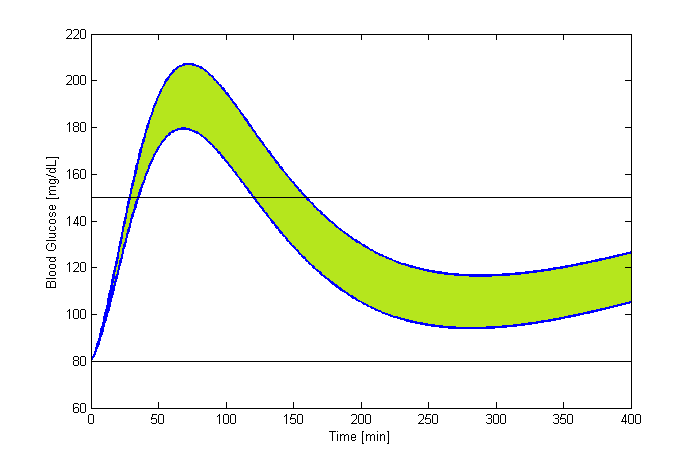
\epsfig{file=Figures/interval.png, width=\textwidth}\caption{Envelopes obtained for an interval simulation of a postprandial period. The simulation considers a 10\% uncertainty in the meal size. The interval bounds are plotted in blue, and the scalar simulations are drawn in green.}
\label{fig:intervalenvelope}
\end{figure}

Intervalization of a given scalar-based model is not straightforward. The computation of both envelopes has to be taken in consideration and depending on the nature of the parameters considered uncertain, the calculations involved can be very complex. Fortunately, interval counterparts of every model proposed in Chapter \ref{sec:ModelsForDiabetes} can be found in literature. In this thesis the intervalization of glucose models will not be reviewed, and instead, it will be taken as given. An extensive review of the models proposed in here was performed by Maria Garcia-Jaramillo in her PhD thesis \cite{mairathesis}, including the intervalization process of every equation and the final interval system of equations of every model. More recently, the model simulated in Figure \ref{fig:intervalenvelope} (model will be reviewed in detail in later chapters) was further improved in its interval form by de Pereda \textit{et al.} \cite{de2012prediction}, including the possibility of simulating as intervals more parameters than the interval version presented by Garcia-Jaramillo. Both versions of the model will be mentioned in the present thesis.

In the rest of this chapter, optimal experiment design and identifiability improvement will be reviewed. Then the interval identification process will be described, including a review of the most used identification algorithms in literature. Finally the optimization tools and software in this thesis will be quickly stated.

\section{Optimizing Identifiability}
\label{sec:Optimizationofidentifiability}

Identifiability analysis can be divided into two stages \cite{walter1997}: \textit{A priori} identifiability and \textit{A posteriori} identifiability. \textit{A priori} identifiability is the feasibility of identification of the model's parameters considering that infinite noise-free data is available. It is an structural property of the model and the lack of it represents a model that can produce the same output with several sets of parameters given a determined input. \textit{A posteriori} identifiability incorporates the data into the identifiability analysis. It analyzes the influence of data noise and uncertainty in the estimation of parameters, and its main outcome is the reliability of an identification.

\subsection{Methods based on FIM}
\label{sec:MethodsBasedOnFIM}

\textit{A posteriori} identifiability often relies in the analysis of the model's parameters sensitivities to the output variations. In the following, the classic method based on the Fisher Information Matrix will be reviewed. Analyzing with detail the Fisher Information Matrix (FIM), all information about \emph{local} identifiability of the model can be extracted, since it implies linearization of the model.

To understand the method, let us take the index defined in equation \eqref{eq:quadraticindex}. The statistical expectation of the index for a set of parameters slightly different than the optimal is given by:

\begin{equation}
	E[J(p+\delta p)]\cong \delta p^{T}\left[\sum_{i=1}^{N}{(\frac{\partial z}{\partial p}(t_{i}))^{T}Q_{i}(\frac{\partial z}{\partial p}(t_{i}))}\right]\delta p + \sum_{i=1}^{N}{tr(V_{i}Q_{i})}
\label{eq:indexdiff}
\end{equation}

where $V_{i}$ represents the covariance matrix of the measurement errors ($Q_{i}$ is typically chosen as $V_{i}^{-1}$), $z$ is the model output and $N$ is the number of data samples. The term between brackets is the Fisher Information Matrix and it expresses the quantity of information contained in the experimental data, as explained in detail by Ljung \cite{ljung1999system}:

\begin{equation}
	FIM=\sum_{i=1}^{N}{\left(\frac{\partial z}{\partial p}(t_{i})\right)^{T}Q_{i}\left(\frac{\partial z}{\partial p}(t_{i})\right)}.
\label{eq:FIM}
\end{equation}

The terms $\partial z /\partial p$ are the sensitivity functions of each parameter $p$ and they are of great importance for the evaluation of the practical identifiability since they gather the parameter influence on the output of the system. The FIM is a square matrix with dimension equal to the number of parameters that are to be identified. The inverse of the FIM is an approximation of the covariance matrix of the estimation error of the model parameters:

\begin{equation}
	C=FIM^{-1}=\left[\sum_{i=1}^{N}{(\frac{\partial z}{\partial p}(t_{i}))^{T}Q_{i}(\frac{\partial z}{\partial p}(t_{i}))}\right]^{-1}
\label{eq:BLUE}
\end{equation}

The diagonal of $C$ contains the information of the confidence interval in the estimation of every parameter. The statistical expected value of the error of an estimation (which is a measure of the confidence interval of the model's parameters) is actually bounded by the matrix $C$ following the Cramer-Rao inequality for unbiased estimators (the true value of the parameters equals the expectation of the estimated parameters), as introduced originally in the classic references \cite{cramer1946mathematical} and \cite{rao2009linear}. 

\begin{equation}
	E \left( \left[ \hat{p}-p\right]\left[ \hat{p}-p\right]^{T}\right) \geq C
\label{eq:CRineq}
\end{equation}

where $E$ stands for the statistical expected value and $\hat{p}$ is a estimation of the parameters $p$. For further explanations and proofs of the Cramer-Rao inequality, the reader is referred to Ljung's work \cite{ljung1999system}. Given that the FIM is known and that it is invertible (non-invertability means structural non-identifiability), the coefficient of variation (CV) for the parameter $p_{i}$ being identified is calculated as:

\begin{equation}
	CV_{i}=\frac{\sqrt{C_{ii}}}{p_{i}}
\label{eq:CR}
\end{equation}

The interpretation of this confidence interval limit is simple: if, for example, a parameter $p_{i}$ has a CV of $0.4$ it means that, for the measurement error which variance was considered in the calculation of $Q_{i}$, successive parameter estimations will have a standard deviation of 40\% of the true parameter value (for a fully efficient unbiased estimator). There is more useful information to be drawn off the FIM, like the correlation matrix. This matrix, the elements of which are the approximated coefficients of correlation between the $i^{th}$ and the $j^{th}$ parameters, is defined as:

\begin{equation}
	R_{ij}=\frac{C_{ij}}{\sqrt{C_{ii}C_{jj}}}
\label{eq:FIMcorrelation}
\end{equation}

Analyzing the correlation matrix gives information on the compensation effect of the changes in the values of the parameters over the model output. If two parameters, $p_{i}$ and $p_{j}$, are highly correlated, a change in the output due to a change in parameter $p_{i}$ can be hidden by the appropriate change in $p_{j}$. Very strong correlations between different parameters are a display of poor identifiability of a model. A correlation of value 1 between parameters is a sign of a structural problem of identifiability of the model, because both parameters have the same exact effect on the model's output. Thus, FIM analysis can also be used in the process of \textit{a priori} identifiability analysis by identifying structural identifiability problems.

\subsection{Monte-Carlo methods}
\label{sec:MonteCarloMethods}

Calculation of the coefficients of variation and the confidence region of the parameters in an identification using the FIM is an approximation of the ``real'' confidence in the parameter's identification. Further methods are explored in literature to obtain better approximations of the CV without incurring in too many approximations. The group of methods for parameter uncertainty estimation that make less assumptions on the parameters distribution is the group of Monte-Carlo methods.

Parameter estimation using data collected from a system will generally not yield the same results if the experiment is repeated, because of the perturbations acting on the system and noise in the measurement systems. The vector of outputs of the system is then a random vector $y^s$ that is related to an estimation of the parameters $\hat{p}(y^s)$. Monte-Carlo methods aim to estimate $\hat{p}(y^s)$ and its confidence region by creating a set of fictitious data vectors with a mathematical model and incorporating realizations of random variables in order to simulate the influence of noise and perturbations, creating the \emph{virtual dataset} $y^m$. Several realization runs of the model applied to different realizations of the ``noise'' will create different estimations $\hat{p}(y^m)$ of the parameter vector.

One of the difficulties of the Monte-Carlo methods lies in the choice of the distribution used to generate the fictitious data $y^m$. The \textit{jack-knife} \cite{quenouille1949approximate} and the \emph{bootstrap} \cite{efron1982jackknife} methods make it possible to avoid estimating the distribution of the noise from the residuals.

\subsubsection{Jack-knife}
\label{sec:JackKnife}

The main advantage of this approach is its simplicity. The virtual data is fragmented in $n_t$ vectors of equal size $y^m_i, (i=1, \ldots , n_t)$. Let $\hat{p}$ be the estimate of the parameters obtained from all the virtual data vector, and $\hat{p}_i$ the estimator related to all the data but $y^m_i$. Then $n_t$ pseudo-estimates can be defined as

\begin{equation}
	\tilde{p}_i=n_t \hat{p} - (n_t -1) \hat{p}_i \quad (i=1, \ldots , n_t)
\label{eq:jackknifepseudo}
\end{equation}

And the computation of the average of these pseudo-estimates is the jack-knife estimator of $\hat{p}(y^s)$, denoted as $p_{jk}$. The covariance matrix of the population of pseudo-estimators $\tilde{p}_i$ is

\begin{equation}
	C_{jk}= \frac{1}{G-1}\sum_{i=1}^{n_t} (\tilde{p}_i-p_{jk})(\tilde{p}_i-p_{jk})^T
\label{eq:jackknifecovariance}
\end{equation}

And the $100(1-\alpha)\%$ confidence interval for a given $p_i$ parameter can be calculated using the $T^2$ Hotelling distribution:

\begin{equation}
	p_{jk_i}\pm t^{1-(\alpha/2)}_{N-N_p}\sqrt{\frac{C_{jk_{ii}}}{n_t}}
\label{eq:jackknifeconfidence}
\end{equation}

where $C_{jk_{ii}}$ are diagonal elements of $C_{jk}$ and $p_{jk_i}$ is the $i$\textsuperscript{th} element of $p_{jk}$.

\subsubsection{Bootstrap}
\label{sec:Bootstrap}

This approach assumes that the errors are independent random variables with identical but otherwise unspecified distribution. In order to obtain an estimation of the parameters $\tilde{p}$, this method uses only the experimental values $y^s$ and the model simulated output values $y^m$. Let us assume

\begin{equation}
	y^s(t_i)=y^m(t_i,p^{*})+b_i \quad (i=1, \ldots , n_t)
\label{eq:bootstrapy}
\end{equation}

where $p^{*}$ is the real value of the parameter vector, and $b_i$ correspond to independent random variables with the same distribution. Then, an estimate of $b_i$ is given by the $i$\textsuperscript{th} residual:

\begin{equation}
	\hat{b}_i = y^s(t_i)-y^m(t_i,\hat{p}) \quad (i=1, \ldots , n_t)
\label{eq:bootstrapbi}
\end{equation}

where $\hat{p}$ is the estimate of the vector $p*$. A vector of virtual data $y^f$ is then obtained as

\begin{equation}
	y^f(t_i)=y^m(t_i,\hat{p})+\hat{b} \quad (i=1, \ldots , n_t)
\label{eq:bootstrapyf}
\end{equation}

where $\hat{b}$ is chosen among the residuals $\hat{b}_k; \; (k=1, \ldots , n_t)$ for every $t_i$ with equal probability for every $\hat{b}_k$. This is equivalent to substituting the empirical distribution of residual for the true distribution of the $b_i$'s, which is more acceptable the closer $\hat{p}$ is to $p*$. Repeating this operation for different runs of the model, a population of fictional vectors of data can be obtained, and similarly to the jack-knife approach, the mean of the population ($p_B$) and the covariance matrix ($C_B)$ can be used to deduce a $100(1-\alpha)\%$ confidence interval for the parameter $p_i$ as follows:

\begin{equation}
	p_{B_i}\pm t^{1-(\alpha/2)}_{N-N_p}\sqrt{C_{B_{ii}}}
\label{eq:bootstrapconfidence}
\end{equation}

where $C_{B_{ii}}$ are diagonal elements of $C_{B}$ and $p_{B_i}$ is the $i$\textsuperscript{th} element of $p_{B}$.

\subsection{Practical Identifiability and Optimality}
\label{sec:PracticalIdentifiability}

Monte-Carlo methods for uncertainty estimation can be too cost effective for large datasets and models, such as those present in the work developed in this thesis. Therefore, FIM based methods for identifiability calculation are used in this thesis from this point onward.

In practical terms, the identifiability analysis must be done applying some simplifications. The sensitivities of the parameters have to be calculated by approximating the derivatives of the output with first order approximations. In general, application of the analytic expression of the derivative function is the correct way of performing the FIM calculation. Regarding the models of diabetes in literature though, the analytical expression of the derivative with respect to the parameters of the model's output is not feasible.

Usually, the sensitivity function is calculated by linearizing the model around the nominal parameter, and obtaining the symmetric first order difference. In practice, two simulations of the model are calculated, one with a positive variation of the selected parameter, and the other with a negative variation and then the sensitivity function, resulting in practice in a linearization of the derivative. The sensitivity function is computed using equation \eqref{eq:Slinearization}.

\begin{equation}
	S_{p}=\frac{z(p+\Delta p)-z(p-\Delta p)}{2\cdot \Delta p}
\label{eq:Slinearization}
\end{equation}

Also, if the FIM results to be singular it can not be inverted, and that is considered a sign of non-identifiability. In fact, it is a sign of \textit{a priori} non-identifiability, so \textit{a priori} identifiability analysis is being carried out with this method as well. Usually, when working with noisy measurements, it is really difficult to get a singular FIM, and yet it will be difficult to identify any parameter because the FIM is bad-conditioned. The condition number of the FIM has to be analyzed to overcome this computation problem, and its magnitude checked to analyze if it permits inversion of the matrix and therefore identifiability of the model.

Identifiability of a model depends on model structure, and the data used for identification. Identifiability of a model can be improved by conditioning the data used for identification, and designing optimal experiments for the model used. So far, identifiability has been analyzed as a property of a parameter, quantified as the confidence interval in the estimation of each parameter. That information is obtained from the Fisher Information Matrix (or better, from its inverse), which summarizes the information of all the parameters of the model for a given experiment. The problem of optimal experiment design can be expressed then as an optimization problem of finding the minimum value of a certain scalar function of the FIM that optimizes the identifiability of the model. That scalar function is called optimality criteria, and its general expression is:
\begin{equation}
	j(\Xi)=\phi[FIM(p, \Xi)] \\
\label{eq:index}
\end{equation}
where $\phi$ is a scalar function. The evaluation of the Fisher Information Matrix is a function $FIM$ of $p$, the parameters vector, and $\Xi$, the experiment conditions to be optimized.

There are several criteria that can be used in this case, as seen in \cite{franceschini2008model}:
\begin{itemize}
	\item D-optimality, in which the scalar function chosen is the determinant of the FIM. The three following equations are equivalent, and all of them define the D-optimality criterion and whether it has to be maximized or minimized in order to improve identifiability:
	\begin{align}
		\Xi &= argmin_{\Xi} \: det(FIM^{-1}(p, \Xi)) \label{eq:Doptimality1} \\
		\Xi &= argmax_{\Xi} \: det(FIM(p, \Xi)) \label{eq:Doptimality2} \\
	  \Xi &= argmax_{\Xi} \: ln(det(FIM(p, \Xi)) \label{eq:Doptimality3}
	\end{align}
	\item E-optimality, in which the function is the smallest eigenvalue of the information matrix, and it has to be maximized.
	\item A-optimality, in which the problem is solved by maximizing the trace of the information matrix.
\end{itemize}
In order to better understand the meaning of these criteria a geometrical analogy is needed. If every parameter is placed in an axis of the geometrical space, then the region defined by the confidence intervals of each one of the parameters defines an ellipsoid the axis of which are given by the eigenvalues of the inverse of the information matrix. Given that the objective of the optimization is to minimize all the regions of confidence, every axis of the ellipsoid have to be minimized, or equivalently, the volume of the ellipsoid has to be minimized, and that volume is exactly the determinant of the inverse of the FIM. The rest of the criteria have similar meanings that are summarized in Figure \ref{fig:criteria}.

\begin{figure}[hbtp]
\centering
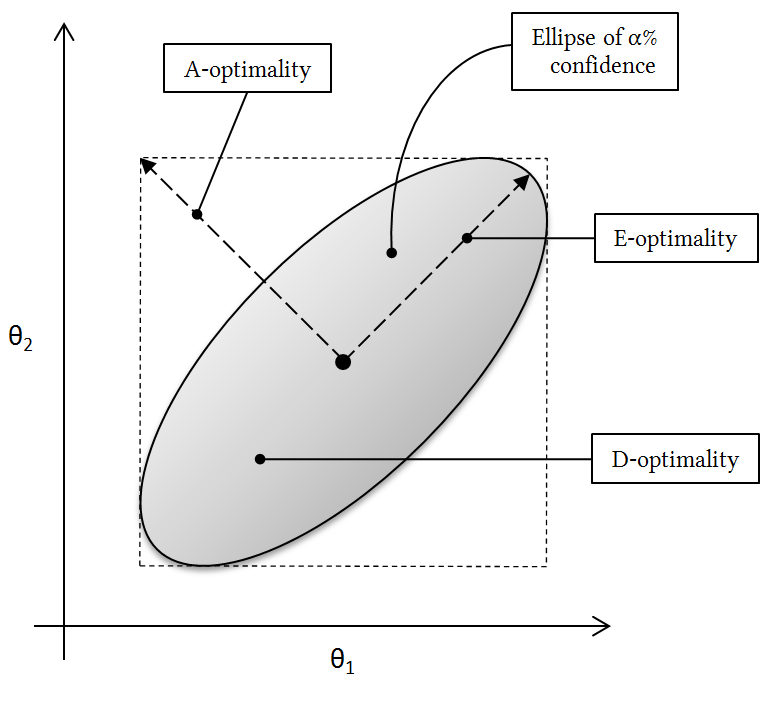
\epsfig{file=Figures/optimalcriterion.png, width=0.7\textwidth}\caption{Each criterion reduces the confidences intervals attempting to minimize one singular scalar value. Adapted from \cite{franceschini2008model}.}
\label{fig:criteria}
\end{figure}

The question of which criterion should be used arises now. The D-optimality is the most used of the three standard criteria cited above. This is due to some exclusive appealing properties of the criterion \cite{franceschini2008model}:
\begin{itemize}
	\item Easy geometrical interpretation, as seen in Figure \ref{fig:criteria}.
	\item Invariance with respect to non-degenerated transformation applied to the model parameters, such as rescaling. This property is applied in equation \ref{eq:Doptimality3} in order to work, during the optimization process, with smaller quantities.
	\item Yielding to optimal experiments which correspond to replications of a small number of different experimental conditions.
	\item Optimal experiment design yields to non-singular FIM.
\end{itemize}
The main drawback this criterion has is that it gives too much importance to the parameter to which the model is most sensitive. Geometrically, this problem is equivalent to the idea of trying to minimize the volume of the ellipsoid by reducing mostly its bigger axis.

There are other criteria available for different purposes, like the modified E-optimality, that tries to maximize the FIM condition number, aiming to make the confidence ellipsoid as spherical as possible \cite{versyck1998optimal}. The correct application of this criterion would be in a case of strong parameter correlations, and the design will yield to a decoupled identification in parameters. That is not the case in this thesis though. D-optimality will be the one used for the experiments designed for diabetic patients, and for every model tested.

The optimization problem associated is non-linear, and global solvers are suggested for its solution. The choice of experimental parameters for the optimization is as wide the experimentation ambit. One of the most common choices is to optimize the sampling times of a given experiment. The choice of these parameters usually relies on the person performing of the experiment design, but it conditions the characteristics of the optimization. Too many parameters may lead to long, unrealistic convergence times on the optimization algorithm, or even non convergence at all. Also, if many experimental parameters are introduced experimental setup may be too complicated to perform. Given this arguments, and especially in the diabetes context, the number of parameters to be optimized should remain as low as possible for achieving the maximum identifiability needed.

\section{Identification with Uncertainty}
\label{sec:IntervalIdentification}

The use of intervals for identification has been developed since the 1990s due to its ability to cope with uncertainty either in the structure of the model and also in the measurements and parameters. Focusing on the measurement error, a parameter estimation methodology outstands over all others: the error-bounded estimation.


\subsection{Error-bounded Estimation}
\label{sec:ErrorBoundedEstimation}

Error bounded estimation assumes that an error exists in the measured variable, and that there exist a trusted estimation of this error. The estimated error must be within bounds that are acceptable for the good working of the system. One may define the error as:
\begin{equation}
	e(p)=\tilde{y}-y(p)
\label{eq:output_error}
\end{equation}
where $\tilde{y}$ is the vector of experimental measurements, and $y(p)$ is the model output, which is dependent on the parameter vector $p$. The problem of bounded error estimation considers that the output errors lie within acceptable bounds:
\begin{equation}
	e^{-} \leq e(p) \leq e^{+}
\label{eq:error_bound}
\end{equation}
where $e^{-}$ and $e^{+}$ are the lower and upper acceptable bounds of the error. The identification problem relies on finding all possible values of the parameter vector $p$ that produce outputs that fall within the acceptable bounds. The subsequent problem is a set inversion problem, and it can be solved by set inversion algorithms like the SIVIA (Set Inversion Via Interval Analysis) algorithm presented in Jaulin \textit{et al.} \cite{jaulin2001applied}.

The SIVIA algorithm divides the parameter space into ``boxes'', i.e multidimensional intervals, and evaluates the correspondent image in the output space for compliance with the desired characteristics. Given that interval analysis produces guaranteed solutions of the output of the model to all the values of the parameter space inside the evaluated box, classification of the boxes evaluated can be divided into three categories:
\begin{itemize}
	\item Guaranteed solutions. All parameters in the evaluated box lead to an output error fulfilling the constraints.
	\item Guaranteed non-solutions. All parameters in the evaluated box lead to an output error violating the constraints.
	\item Indeterminate solutions. Otherwise.
\end{itemize}
The algorithm works iteratively classifying the boxes into these three categories and dividing indeterminate boxes into smaller boxes for further classification. The algorithm searches all the parameter space. The accuracy of the algorithm is given by the acceptable size of the indeterminate boxes in the parameters space. These boxes compose the boundary of the parameter space that produces outcomes of the model in the acceptability constraints.
\begin{figure}[hbtp]
\centering
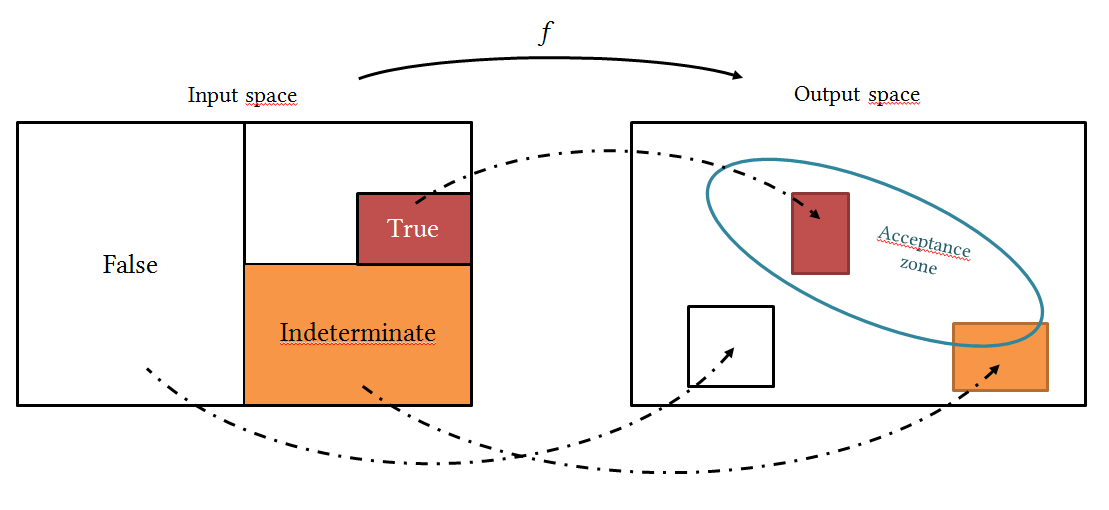
\epsfig{file=Figures/sivia.png, width=\textwidth}\caption{Basics of the SIVIA algorithm. The boxes that produce images in the output space that fall within the acceptability range (red ellipse) are classified as true solutions, in blue. Boxes out of the acceptability zone are classified are false solutions and marked in white. Red boxes are undetermined. Adapted from \cite{jorgeibolus}}
\label{fig:sivia}
\end{figure}
The SIVIA methodology is summarized in Figure \ref{fig:sivia}. The images in the output space are related to boxes in the input (or parameter) space. The boxes in the input space are divided each time they are classified as undetermined. The first evaluation to be performed correspond to the whole parameter space, which will be evaluated as undetermined if the acceptability criterion embraces only some part of the output space. The parameter space is then divided using a predefined criterion to the choice of the user into smaller boxes, and reevaluated. The algorithm then works as a tree-search algorithm, finishing a branch when it is classified into true or false solutions, or if the resolution threshold for the search boxes is met.
%A classic example of the performance of error-bounded estimation will be reproduced next in order to better display this set inversion problem. A simple two parameter model is to be fit to data with consideration of uncertainty in it. The data for the example was first found in \cite{milanese1991estimation}. The model to be fit responds to the equation:
%\begin{equation}
%	y(p_{1},p_{2},t_{i})=20 \exp(-p_{1} \, t_{i})-8 \exp(-p_{2} \, t_{i})
%\label{eq:error_bound_ex}
%\end{equation}
%where $p_1$ and $p_2$ are the parameters to be identified with uncertainty. The data for the identification was sampled at different times, and it presented different relative error known \textit{a priori} following $[e]=[-e_{max},e_{max}]$ with $e_{max}=0.5\left|\tilde{y}\right|+1$, where $[e]$ is the vector of acceptable intervals for the error and $\tilde{y}$ are the experimental measurements. Notice that the error estimation is considered as given for the problem. The vector of sampling times and related experimental measurements with the error interval associated to each sample are displayed in Table \ref{tab:error_bounded_example}. The same samples are displayed in Figure \ref{fig:error_bounded} in a Cartesian plot for easier visualization of the problem.
%\begin{table}[hbtp]
%	\centering
%		\begin{tabular}{|c c c|}
%		\hline 
%		$i$ & $t_{i}$ & $\tilde{y}$ \\
%		\hline 
%		$1$ & $0.7$ & $[2.7, 12.1]$ \\
%	  $2$ & $1.5$ & $[1.04, 7.14]$ \\
%		$3$ & $2.25$ & $[-0.13, 3.61]$ \\
%		$4$ & $3$ & $[-0.95, 1.15]$ \\
%		$5$ & $6$ & $[-4.85, -0.29]$ \\
%		$6$ & $9$ & $[-5.06, -0.36]$ \\
%		$7$ & $13$ & $[-4.1, -0.04]$ \\
%		$8$ & $17$ & $[-3.16, 0.3]$ \\
%		$9$ & $21$ & $[-2.5, 0.51]$ \\
%		$10$ & $25$ & $[-2, 0.67]$ \\		
%		\hline 
%		\end{tabular}
%	\caption{Measurement times and corresponding interval data.}
%	\label{tab:error_bounded_example}
%\end{table}
%\begin{figure}[hbtp]
%\centering
%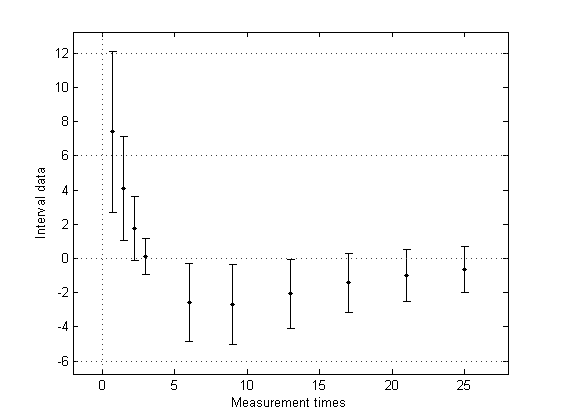
\epsfig{file=Figures/errorbounded.png, width=\textwidth}\caption{Acceptable data measurements including data uncertainty displayed as vertical bars (extracted from \cite{milanese1991estimation}).}
%\label{fig:error_bounded}
%\end{figure}
%The error bounded identification for this data-set is defined as the set of parameters $p_1$ and $p_2$ that create curves from equation \eqref{eq:error_bound_ex} that cross all the vertical bars in Figure \ref{fig:error_bounded}, which represent the experimental values. The set of solutions from the error-bounded identification then represents all possible model outcomes that are compliant with the error estimation considered. The solution set in the parameter space is shown in Figure \ref{fig:error_bounded_solution}. The thinner boxes represent the boundary of the optimization algorithm where the resolution threshold was met. All the boxes within the boundary are guaranteed solutions to the problem, and the boxes out of the boundary are guaranteed not to be solutions.
%\begin{figure}[hbtp]
%\centering
%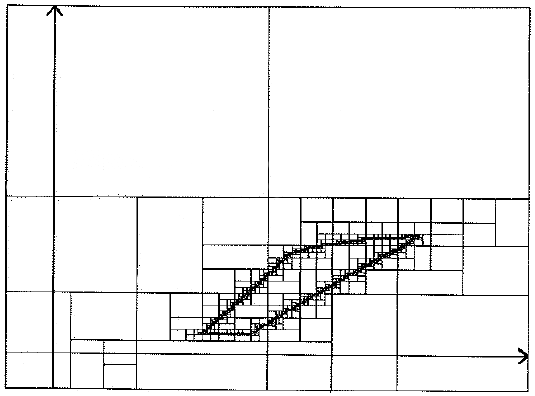
\epsfig{file=Figures/error_bounded_ex_solution.png, width=0.7\textwidth}\caption{Parameter space for the parameters $p_1$ and $p_2$. The frame corresponds to the search domain $[-0.1, 1]^{2}$ (extracted from \cite{jaulin1993guaranteed}).} 
%\label{fig:error_bounded_solution}
%\end{figure}

Even though error-bounded estimation is very extended within the scientific community, it depends heavily on the estimation of the error assumed in the measurements. In the context of diabetes monitoring, errors associated to continuous glucose monitoring are often very large \cite{mazze2009evaluating} which makes CGM estimations too noisy for a closed loop control environment, given the complexity of the models associated. In the hospital environment is possible to obtain much more reliable measurements, with errors smaller than the 2\% \cite{nowotny2012precision}, which can always be neglected for identification. 

Error-bounded estimation is very much focused in the search of feasibility of a group of parameters with the uncertainty of the measurement, although it can also be used for consideration of parametric variability. For control-oriented identification, finding all possible values of the parametric space in which the model's parameters move (system's variability) is more important than finding the feasible parameter set that matches the uncertainty in the measurement. Therefore, a successful robust controller has to respond to system's variability, but never neglecting the influence of measurement errors.

\section{Software and optimization tools}
\label{sec:OptimizationAndSoftware}

Identification and optimization is usually a computationally intensive task. Global non-convex optimization is especially demanding in computation requirements, and it has been established that identification on model identification in diabetes relies on global optimum solutions. There is a wide variety of optimization methods available in literature, but in the following lines we will quickly review the algorithms to be used in this thesis.

All data analysis and computations were done in the Matlab environment, release 2012a (Mathworks, Natick, MA).

\subsection{Scatter search for Matlab}
\label{sec:ScatterSearchForMatlab}

Scatter search for Matlab (SSM from now on) is a global optimizer based on statistical principles and geometrical analysis of the parameter space. This search algorithm has already been used in the artificial pancreas environment with the objective of patient identification, by Cesar Palerm in Santa Barbara \cite{palerm2006robust}.

SSM optimizer is a project of the CSIC (Centro Superior de Investigaciones Cientificas) and the University of Vigo. It is a global optimizer, easily comparable with genetic algorithms. However, SSM does not use codification of the population as genetic algorithms do, although it does work by spawning new generations (offspring) of the function optimum by combining the properties of the previous (parents) population. SSM does not generate random ``mutations'' on the population, as opposed to genetic algorithms, although it renews the existing individuals by adding new random samples to the new generations of optimal solutions in each algorithm iteration. For the details of the inner working of the algorithm, information on the computational cost and better understanding of the searcher the reader can refer to Julio Banga's group papers in 2006 \cite{rodriguez2006novel} and 2007 \cite{egea2007scatter}.

This optimizer has the advantage of using local solvers to refine the search when it seems to have found some optimum solution. The local solver to be used can be chosen from a list available in the SSM's documentation. The local solver chosen was the \textit{fmincon} solver, which is implemented in Matlab's Optimization Toolbox, along with many other optimizers and aid tools for solving any optimization problem in the Matlab environment. This local solver fits into the group of solvers denominated as ``Nonlinear programming solvers'', or ``Constrained nonlinear optimizers''. This sort of algorithms are deterministic solvers that use first and second derivatives of the objective function, along with some heuristics to cope with the various problems that deterministic local searchers have. Abundant information about this kind of algorithms can be found in Coleman and Li paper of 1996 \cite{coleman1993interior}, Powell's conference in 1978 \cite{Powell1978NLSQP}, or for a more general reference see Bazaraa's book \cite{bazaraa2006nonlinear}.

\subsection{Covariance Matrix Adaptive Estimation}
\label{sec:CovarianceMatrixAdaptativeEstimation}

A very well known global optimization method within the scientific community is the algorithm of estimation based on adaptations of the matrix of covariance of the sample population (CMAES). CMAES performs very fast optimizations on a single objective even for large parameters spaces. The optimization performed by CMAES is based on the update of generations of sampling individuals, in a similar way as an evolutionary algorithm, although the update process and the randomly generated individuals are handled differently.

CMAES uses statistical properties of the populations and updates them in each iteration based on the characteristics of the population and the explored parameter space. The adaptation objective in on the covariance matrix adaptation moves the sampling population in order to better fit it to the contour lines of the objective function being minimized. It is assumed that the optimal covariance matrix equals the inverse of the Hessian matrix, although this is only strictly true in convex-quadratic functions. For general optimization functions, the CMAES methodology aims to approximate the inverse of the equivalent of the Hessian matrix for the objective function properties. Convergence and performance of this family of algorithms can be accessed in the proceedings of the 2005 IEEE Congress on Evolutionary Computation \cite{auger2005restart}. For further explanation on the CMAES rational, and its computational analysis, the reader is referred to the works of Hansen in \cite{hansen2006cma} and \cite{hansen2004evaluating}.

Optimizations using interval parameters may consist of two independent parameter sets, upper and lower bounds, where obviously all the lower bounds must be smaller than their respective upper bounds. These greater-or-equal restrictions introduce further constraints on the optimization index. Unfortunately, the build released by Hansen \textit{et al.} \cite{hansen2004evaluating} does not implicitly consider restrictions neither in the outputs nor in the inputs, so they have to be integrated in the cost index with a penalty method.

\subsection{$\epsilon$- MOGA Evolutionary Algorithm}
\label{sec:EpsilonMOGAEvolutionaryAlgorithm}

Classic parametric identification results in a single ``optimal'' point in the parameter space, being insufficient for the case of a time-varying model based on poor prediction capabilities. Many problems in engineering can be translated to multiobjective optimization problem, including the diabetic patient identification problem. In the case of identification in presence of uncertainty using interval models, a problem of optimization of two objectives can be suggested: minimization of glucose interval width and minimization of the fitting error. This problem will be explained in detail in the following thesis, and multiobjective optimization algorithms are used to find it's solution. A brief explanation of these kind of algorithms follows, along with the details of one particular methodology used in this work.

Multiobjective identification is the process of simultaneously optimizing two or more conflicting objectives subject to certain constraints. The solution of this kind of problems is not a single optimal point in the objectives search space, but a family of solutions called a Pareto Front (PF). PF present advantages over single objective optimization techniques:
\begin{itemize}
	\item Provide the designer with the possibility of a better selection of the final solution, presenting a wide variety of possibilities that in many cases include the single objective solution of an analog problem.
	\item Are representative of the whole space of design variables, all of them optimal.
	\item Require of no \emph{tradeoff} parameters to be tuned in the algorithm.
\end{itemize}
PF are created on the basis that each individual in the family is non-dominated by the other individuals. An individual is dominated by other in the population if its evaluation in \emph{both} of the optimization objectives is worse. Therefore, an individual is considered non-dominated and included in the PF by the algorithm if it is best solutions for both objectives in a particular region of the objective space i.e. it cannot be replaced by other point in the objective space for improving an objective, without worsening another one. 

\begin{figure}[hbt]
\centering
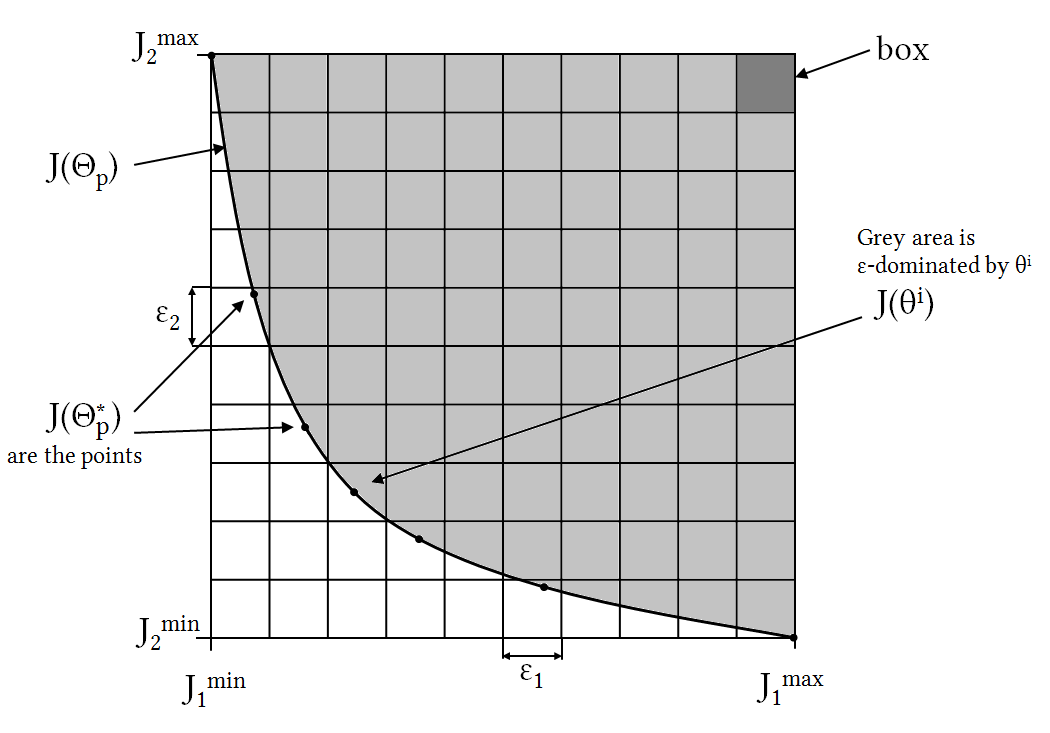
\epsfig{file=Figures/eps_dominance.png, width=0.8\textwidth}\caption{Display of the concept of $\epsilon$-dominance. $J(\Theta_p)$ represents the PF interpolation and $J(\Theta_p^*)$ the actual PF individuals. $J_1$ and $J_2$ are the objective variables, and $\epsilon_1$ and $\epsilon_2$ are the box widths (adapted from \cite{herrero2007well}).}
\label{fig:eps_dominance}
\end{figure}

Evolutionary algorithms are popular solvers for multiobjective problems because of Pareto front groups being susceptible to evolution rules, and both the solver and the problem being population based methods. The $\epsilon$-MOGA (Multi Objective Genetic Algorithm) evolutionary algorithm developed by \cite{herrero2007well} takes the concept of dominance an step further with the notion of $\epsilon$-dominance. $\epsilon$-dominance is based on the domination concept explained before, but it ads a new constraint to the PF individuals: each individual must be isolated within a box of previously defined magnitude. The concept of $\epsilon$-dominance is clearly displayed in Figure \ref{fig:eps_dominance}, where the objective space is overlapping a grid of equally dimensioned boxes. Dominance is then applied to the box in which the Pareto individual is placed, and not just to the point in the objective space. This box-dominance is the $\epsilon$-dominance of the individual of the PF in that box.

The $\epsilon$-MOGA algorithm is able to characterize all kind of PF, including non-convex, non-linear discontinuous search spaces, which is the case for diabetic patient models optimization. The algorithm converges faster than similar evolutionary algorithms, and supposes a smaller computational burden \cite{juanmatesis}. The main achievement of this algorithm is the fact that the PF obtained from $\epsilon$-dominance are well-distributed in the objective space independently of the problem, which is not the case for any other multiobjective optimization algorithm. A well distributed PF is of great help in the interpretation of the results, and can be of utility when choosing an individual out of the PF with a decision making methodology.


